% % Single-row top-of-page figure that fuses what used to be Figure 6
% % (zero-variance ratios on Easy / Hard) and Figure 7 (threshold entropy +
% % Stage 1/2 ablation) into one wide composite.
% %
% % The composite PDF is rendered by
% %   ICML2026-submission-figure-script-drawio-todo/wandb-figure/merge4_zerovar_component.py
% %
% % Sub-labels are produced via \phantomsubcaption from the `subcaption`
% % package, so existing \ref{fig:non-zero-diveregence-comparison},
% % \ref{fig:gamma_entropy} and \ref{fig:ablation} keep resolving — and we
% % additionally expose \ref{fig:zerovar_easy} / \ref{fig:zerovar_hard}.

% \begin{figure}[t]
%     \centering
%     \includegraphics[width=\linewidth]{figures/experiment/exp-merge4-zerovar-component.pdf}%
%     %
%     % Phantom sub-labels — invisible.  We anchor each one inside a zero-
%     % width subfigure so the subcaption counter is bumped for the label
%     % that follows it.  After all four panels are claimed, the figure-
%     % level \caption{} step the figure counter so the trailing
%     % \label{fig:non-zero-diveregence-comparison} binds to the figure
%     % number, not the last sub-letter.
%     %
%     \begin{subfigure}{0pt}\phantomsubcaption\label{fig:zerovar_easy}\end{subfigure}%
%     \begin{subfigure}{0pt}\phantomsubcaption\label{fig:zerovar_hard}\end{subfigure}%
%     \begin{subfigure}{0pt}\phantomsubcaption\label{fig:gamma_entropy}\end{subfigure}%
%     \begin{subfigure}{0pt}\phantomsubcaption\label{fig:ablation}\end{subfigure}%
%     %
%     \caption{\textbf{Zero-variance ratios and component analysis.}
%     (a)~Easy zero-variance ratio: HIVE keeps the lowest fraction of all-correct prompts throughout training.
%     (b)~Hard zero-variance ratio: HIVE rapidly drops below DS and tracks GRESO.
%     (c)~The Stage~2 median prompt-entropy threshold $\gamma$ adapts as the policy becomes more confident.
%     (d)~Removing either Stage~1 or Stage~2 worsens the accuracy--rollout tradeoff.\red{replace the figures to pdf}}%
%     \label{fig:non-zero-diveregence-comparison}
%     \vskip -0.08in
% \end{figure}

\begin{figure*}[t]
    \centering
    \begin{subfigure}[b]{0.24\textwidth}
        \centering
        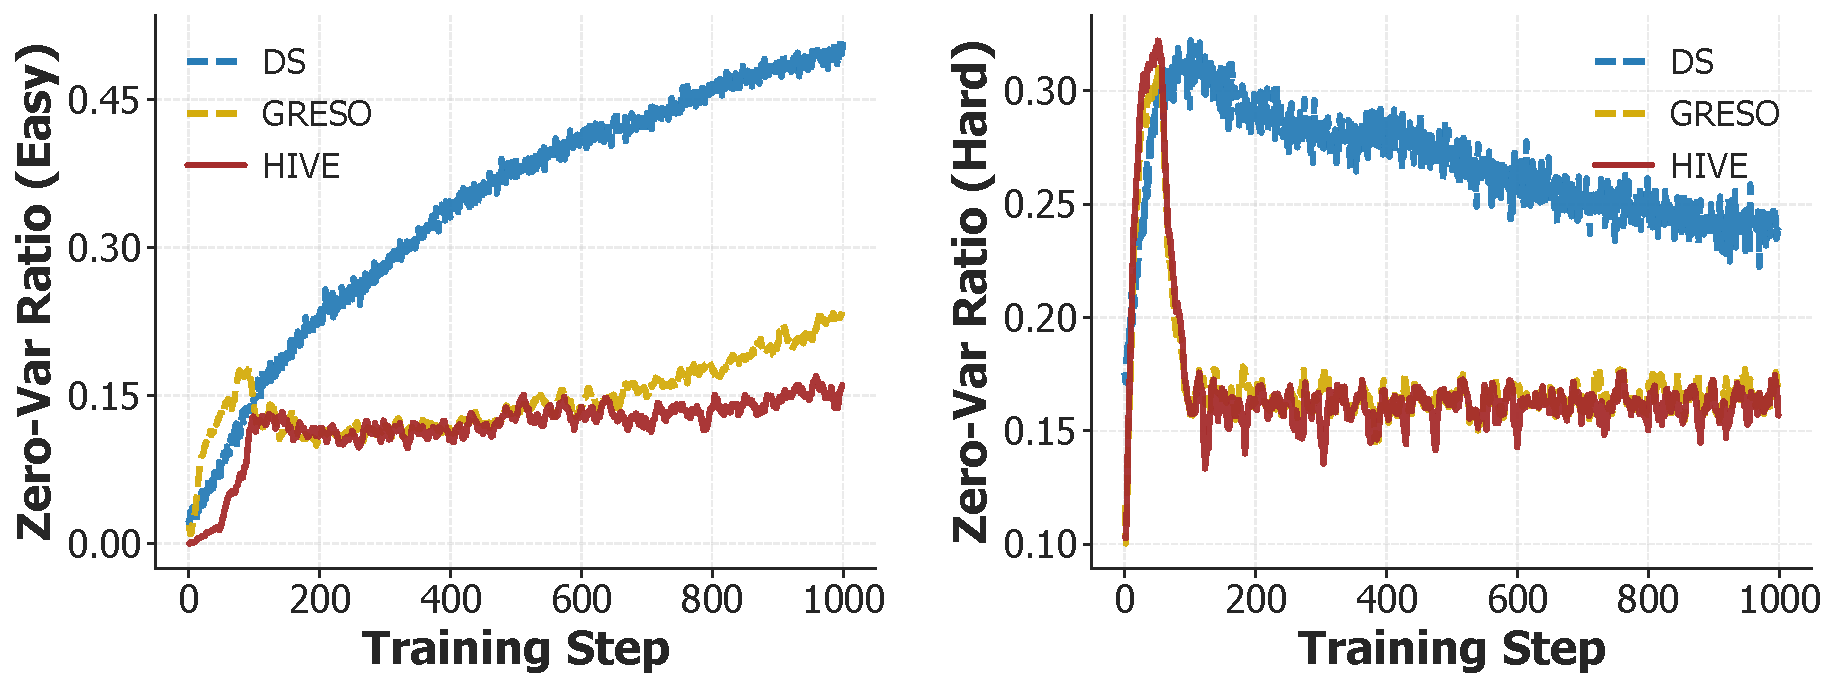
\includegraphics[width=\textwidth,trim=0 0 440.4bp 0,clip]{figures/experiment/fig6-zerovar-easy-hard-polished.pdf}
        \caption{Easy zero-variance}
        \label{fig:zerovar_easy}
    \end{subfigure}
    \hfill
    \begin{subfigure}[b]{0.24\textwidth}
        \centering
        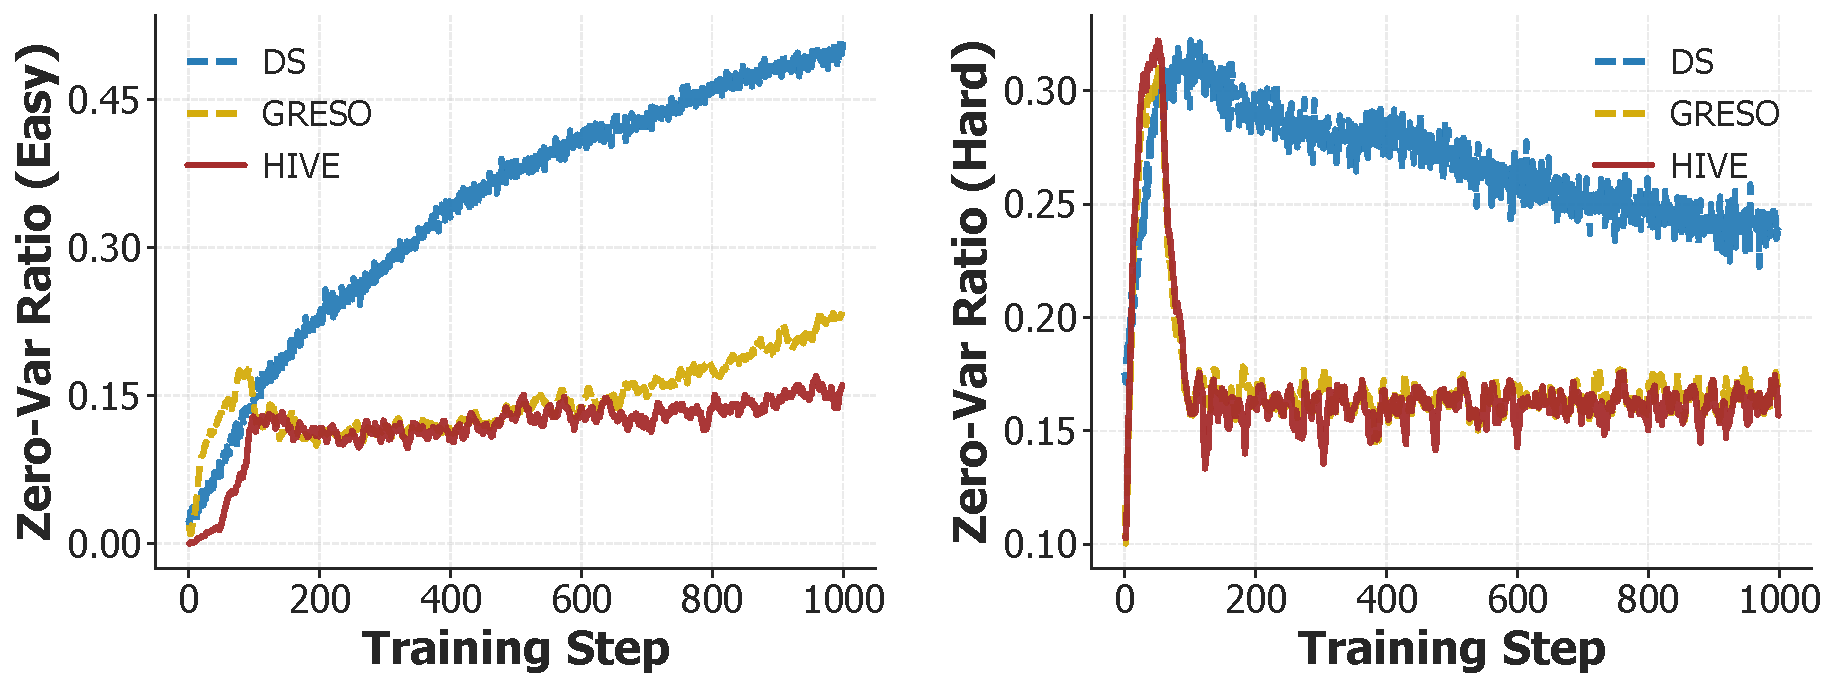
\includegraphics[width=\textwidth,trim=440.4bp 0 0 0,clip]{figures/experiment/fig6-zerovar-easy-hard-polished.pdf}
        \caption{Hard zero-variance}
        \label{fig:zerovar_hard}
    \end{subfigure}
    \hfill
    \begin{subfigure}[b]{0.24\textwidth}
        \centering
        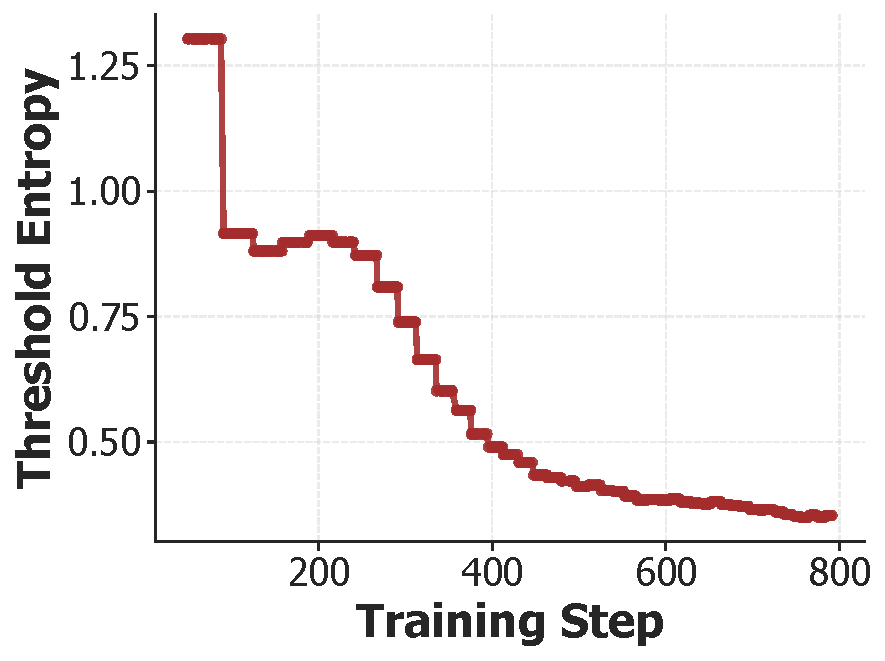
\includegraphics[width=\textwidth]{figures/experiment/fig6-gamma-entropy-polished.pdf}
        \caption{Entropy threshold}
        \label{fig:gamma_entropy}
    \end{subfigure}
    \hfill
    \begin{subfigure}[b]{0.24\textwidth}
        \centering
        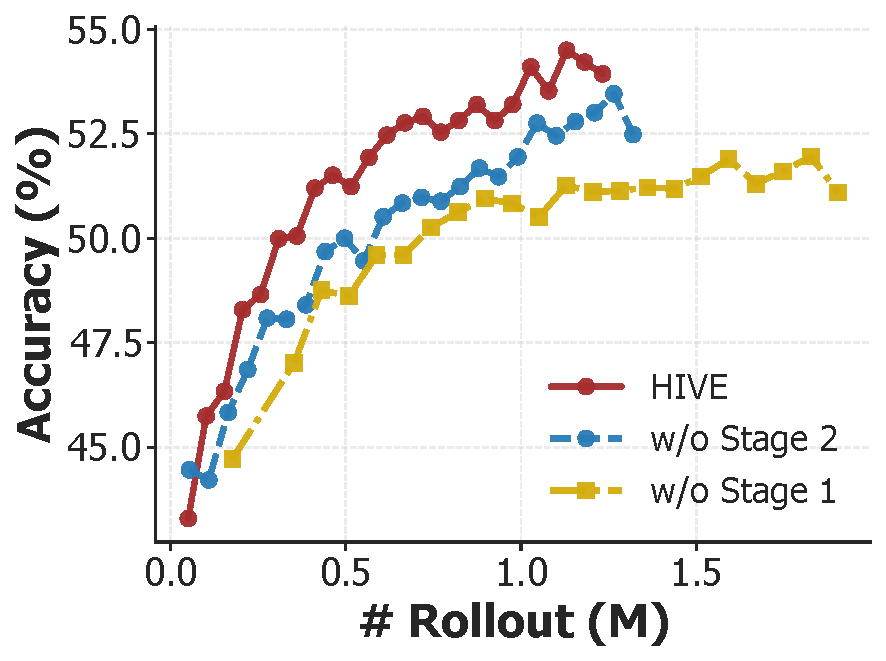
\includegraphics[width=\textwidth]{figures/experiment/fig6-stage-ablation-polished.pdf}
        \caption{Stage ablation}
        \label{fig:ablation}
    \end{subfigure}

    \caption{\textbf{Zero-variance ratios and component analysis.}
    (a)~Easy zero-variance ratio: HIVE keeps the lowest fraction of all-correct prompts throughout training.
    (b)~Hard zero-variance ratio: HIVE rapidly drops below DS and tracks GRESO.
    (c)~The Stage~2 median prompt-entropy threshold $\gamma$ adapts as the policy becomes more confident.
    (d)~Removing either Stage~1 or Stage~2 worsens the accuracy--rollout tradeoff.}%
    \label{fig:non-zero-diveregence-comparison}
    \vskip -0.08in
\end{figure*}
